\section{SIFT}
\label{sec:Chapter21}
SIFT - Scale Invariant Feature Transform (tj. Škálově invariantní transformace charakteristik/rysů) představuje jeden z prvních a zároveň klasických metod pro detekci a popis klíčových bodů v obrázcích, jak bylo poprvé popsáno v literatuře \cite{sift}. Tento algoritmus je navržen tak, aby automaticky identifikoval a popsal velké množství klíčových bodů v různých škálách vstupního obrázku, což může dosáhnout počtu v řádech tisíců pro obrázky s rozměry přibližně 500/500 pixelů. Přesné množství detekovaných bodů závisí na vizuálních charakteristikách a složitosti obrázku.

Pro lokalizaci bodů se používají rozdíly Gaussovy funkce s různými hodnotami sigma ($\sigma$). Tento proces spočívá ve vyhledávání lokálních extrémů v rozdílech mezi sousedními úrovněmi Gaussovy funkce, aplikovanými na obrázek v dané škále obrázku (oktávě). SIFT generuje těchto oktáv několik, každý s jinou velikostí daného původního obrázku. Pro každou oktávu je pak vygenerována sada těchto výsledků Gaussovy funkce ze sad hodnot sigma ($\sigma$). Vizuální reprezentace těchto různých oktáv pod sebou pak následně připomíná pyramidu.

Na základě tohoto přístupu jsou následně klíčové body transformovány do deskriptorů, které jsou robustní vůči změnám škál, rotace a menším změnám úhlu pohledu. Deskriptory klíčových bodů jsou invariantní díky směru vycházejících z charakteristik DoG. Jsou také velmi distinktivní, tzn. vykazující rozdíly oproti ostatním stabilním deskriptorům nalezených na obrázku, což vede k nezaměnitelnosti a následně i například spolehlivé párové identifikaci mezi více obrázky.

\begin{figure}[h]
\centering
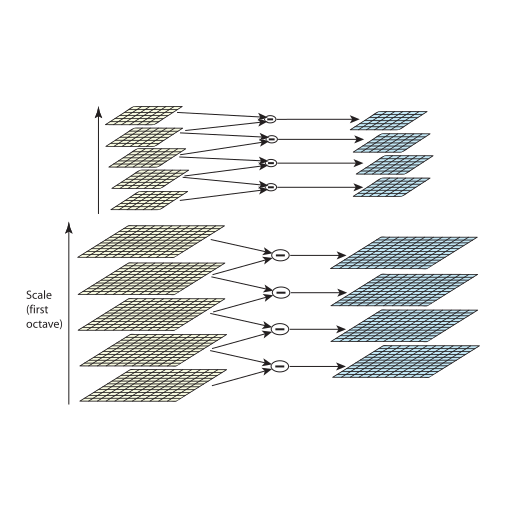
\includegraphics[width=1.0\textwidth,keepaspectratio]{Figures/sift_dog.pdf}
\caption[Vizuální reprezentace výpočtu DoG v metodě SIFT]{Vizuální reprezentace výpočetu DoG v metodě SIFT. Převzato z \cite{sift}.}
\label{fig:sift_dog}
\end{figure}

Tato distinktivnost a robustnost SIFT deskriptorů umožňuje efektivní vyhledávání a párování klíčových bodů mezi obrázky, což je klíčové pro mnoho aplikací v oblasti počítačového vidění, jako je rozpoznávání scén a objektů či sledování pohybu. Díky těmto vlastnostem se SIFT stal základním stavebním kamenem pro mnohé následující výzkumy a aplikace v oblasti rozpoznávání obrazu \cite{sift}.

SIFT však není posledním vývojovým stupněm v technologiích detekce a popisu klíčových bodů. Od jeho vzniku bylo vyvinuto několik dalších algoritmů, které staví na jeho základech nebo se snaží překonat některé jeho omezení. Mezi tyto následující algoritmy patří například SURF (Speeded Up Robust Features) \cite{surf}, ORB (Oriented FAST and Rotated BRIEF) \cite{orb}, a dalších, které se snaží zlepšit rychlost, efektivitu, nebo invarianci k různým transformacím.
\endinput